% 业余无线电通信
% 业余无线电通信.tex

\documentclass[12pt,UTF8]{ctexbook}

% 设置纸张信息。
\usepackage[a4paper,twoside]{geometry}
\geometry{
	left=25mm,
	right=25mm,
	bottom=25.4mm,
	bindingoffset=10mm
}

% 设置字体,并解决显示难检字问题。
\xeCJKsetup{AutoFallBack=true}
\setCJKmainfont{SimSun}[BoldFont=SimHei, ItalicFont=KaiTi, FallBack=SimSun-ExtB]

% 目录 chapter 级别加点(.)。
\usepackage{titletoc}
\titlecontents{chapter}[0pt]{\vspace{3mm}\bf\addvspace{2pt}\filright}{\contentspush{\thecontentslabel\hspace{0.8em}}}{}{\titlerule*[8pt]{.}\contentspage}

% 设置 part 和 chapter 标题格式。
\ctexset{
	chapter/name={第,章},
	chapter/number={\arabic{chapter}}
}

% 图片相关设置。
\usepackage{graphicx}
\graphicspath{{Images/}}

% 设置署名格式。
\newenvironment{shuming}{\hfill\zihao{4}}

% 注脚每页重新编号,避免编号过大。
\usepackage[perpage]{footmisc}

\title{\heiti\zihao{0} 业余无线电通信}
\author{童效勇(BA1AA), 陈方(BA4RC)编著}
\date{}

\begin{document}

\maketitle
\tableofcontents

\frontmatter

\begin{figure}[htbp]
	\centering
	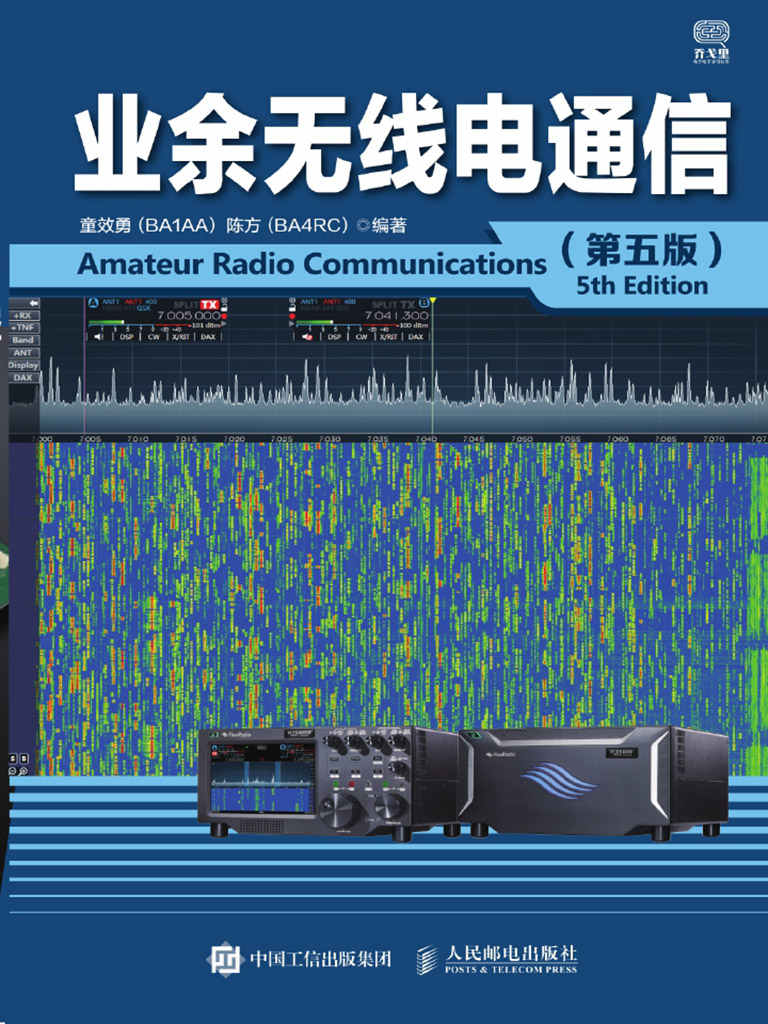
\includegraphics[width=0.7\linewidth]{cover}
	\caption{}
	\label{fig:1}
\end{figure}

\chapter{内容提要}

本书是由业余无线电家童效勇(BA1AA)和陈方(BA4RC)为广大业余无线电爱好者编写的业余无线电通信入门教材。

本书系统地介绍了开设、操作业余无线电台的相关知识和法律法规,主要内容包括:业余无线电通信简史、业余无线电通信操作实践、收发报技术的自我训练、业余无线电奖励证书和竞赛活动、不同业余无线电波段的运用、业余短波天线、业余无线电收发信机、依法设置和使用业余无线电台等。

本书既可作为开展业余无线电活动的教材,也可作为业余无线电爱好者的自修读本和手册。

\chapter{编著者的话}

业余爱好是人类社会进步的产物,是社会文明进步的标志。古今中外大凡发明创造者都有其业余爱好,而伟大的发明出自业余爱好者之手的例子更是不胜枚举。电气研究先驱者富兰克林12岁当印刷学徒并从未离开过印刷业;揭示电磁感应的法拉第也曾是报童、装订工,后来还成为一名化学专业研究者;电报机发明者莫尔斯发明电报时正从事大学的工艺美术教学……科学巨匠爱因斯坦说:“智慧并不产生于学历,而是来自对于知识的终生不懈的追求。”孔子也说:“知之者不如好之者,好之者不如乐之者。”不要被拜金主义、享乐主义和其他世俗的观点淹没了你的兴趣、爱好和激情!我们的祖国正需要千千万万个爱迪生式的发明家,而当今世界对人才的激烈竞争也正呼唤着每一个有志者从自己的业余爱好中去钻研、去实践、去塑造,以发现崭新的自我。

业余无线电通信活动以其极为丰富的内涵吸引了并将继续吸引着无数爱好者。科技性、先进性、实用性、群众性、国际性使这项活动与其他任何业余兴趣活动有着很大的不同;培养高素质的技术人才,丰富人们的文化生活,为抢险救灾提供有效的通信服务,促进各国人民间的交流,增进友谊,这一切正是改革开放不断深入的中国所迫切需要的。正因为这样,业余无线电通信活动及其标志—业余电台正越来越受到国家和各有关方面的重视,推动发展和加强管理的一系列法规、政策也已日趋完善。

我国有着大量的无线电技术爱好者,但进行业余无线电通信实践的人还不是很多。编写本书的目的是帮助更多的朋友学习和掌握业余无线电通信的基本知识和技能,尽可能地为乐于此道的爱好者们提供一本较为翔实的自我训练的教材。

改革开放的春风已吹绿了中国业余无线电通信芳草地,业余电台正如雨后春笋般出现在神州大地。愿爱好者在这里汲取更多的雨露和阳光,培育出更加绚丽夺目的奇葩—HAM之花!

1995年1月

\chapter{修订说明}

《业余无线电通信》一书自1995年出版以来,历经了数次改版、重印,2016年6月推出的第四版,也已陆续重印了三十余次。这说明在无线电技术和电子科学迅速发展的今天,这本“入门砖”性质的小册子,在广大业余无线电爱好者群体中还有一定的需求量。能够为我国业余无线电的发展尽一份微薄之力,这让我们感到十分欣慰。

为能适应科学技术和社会的快速发展以及业余无线电实践的丰富、进步,《业余无线电通信》先后于2004年、2011年和2015年进行过3次修订,出版了《业余无线电通信》第二版、第三版和第四版。在这几次修订中,除了对正文和附录里一些时效性较强的内容作必要的修改、调整外,改写了第8章《依法设置和使用业余电台》,增加了业余无线电在我国的发展简史,介绍了我国业余无线电爱好者群体在2008年汶川地震抢险救援应急通信工作中的突出表现,增加和改写了部分业余无线电通信操作实践方面的内容。

2020年10月,我们完成了《业余无线电通信》第4次修订。为能使书稿继续与时俱进,更好地服务于广大读者,我们在不改动原书总体结构的原则下,对涉及时效性的叙述及附录再次进行了修改调整,增加了软件无线电通信技术介绍、如何在线学习CW技术等方面的内容,在附录中增加了设计制作业余无线电测向机的相关内容。

《业余无线电通信》的每一次修订,都得到了许多业余无线电组织、业余无线电家和爱好者的帮助,在此一并向他们致谢。衷心感谢中国无线电运动协会,江苏、上海、天津等省、市无线电运动协会,中国无线电协会业余无线电分会以及龚万聪(BA1DU),陈平(BA1HAM),范斌(BA1RB),焦亮梅(BD1AYL),尹虎(BD1AZ),穆新宇(BD1ES),李彬(BA4REB),陈新宇(BA4RF),李家伟(BA4WI),卜宪之(BD4RG),姜锦中(BD4RQ),王龙(BD4RX),薛立人(BA5RX),郑英俊(BA5TX),陈衡(BD5RV/4),刘旭(BA8DX),刘虎(BG8AAS)等HAM在书稿校对、资料提供、翻译、新增内容的撰写等方面所给予的无私帮助,同时也感谢指正原书中的错漏之处并提出修改意见和建议的读者朋友们!

编著者

2020年10月22日

\mainmatter

\chapter{什么是业余无线电通信}

在科学技术迅速发展的今天,无线电通信已经深入到包括人们日常生活在内的各个领域。无论是天上的飞机、卫星,海上的轮船、舰艇,陆地上的各种车辆,还是人们熟悉的收音机、电视机、移动电话、Wi-Fi无线网络……全都离不开无线电通信技术。

业余无线电通信(以下有时简称“业余通信”)是整个无线电通信世界当中一个重要的组成部分。它是一项鼓励人们去从事无线电收信和发信实践的业余兴趣爱好活动。业余无线电通信的英语名字是“Amateur Radio”,符合国际电信联盟ITU定义的业余无线电爱好者是“Radio Amateur”,在世界上又普遍被称为“HAM”。由于“HAM”在英语中被解释为“火腿”,所以“火腿”又成了从事业余无线电通信的爱好者们的另一个名字。

业余无线电通信技术是一项内涵极其丰富的专门技术,所以人们还把获得发信执照、精通业余无线电技术和通信的爱好者称为“业余无线电家”,以区别于一般的电子技术爱好者。业余无线电通信的天地是博大的,当打开自己的收、发信机时,你可以听到来自世界各个角落的HAM的声音。当你获得业余无线电执照后,你可以轻松地和任何一个国家和地区的HAM交谈而无须办理出国护照,也可以从无数不见面的朋友那里得到技术上的支持。你会为自己第一次成功地和远方的朋友通信而兴高采烈,更可能会为自己在电子技术、通信技巧以及语言、人文地理等许多方面知识才能的迅速提高而大吃一惊!到那时,你才会更深切地体会到:业余无线电通信确实是一项遍及全世界的十分有意义的兴趣爱好活动。

\section{什么是业余电台}

联合国下设的专业机构“国际电信联盟”(ITU,International Telecommunication Union)根据不同的用途将全世界所有无线电通信分为若干种“业务”(Service),其中有两种业务用于业余无线电(Amateur Radio):“业余业务”(Amateur Service)和“卫星业余业务”(Amateur-Satellite Service)。ITU对业余业务的定义为“供业余无线电爱好者进行自我训练、相互通信和技术研究的无线电通信业务。业余无线电爱好者系指经正式批准的、对无线电技术有兴趣的人,其兴趣纯系个人爱好而不涉及谋取利润”。对卫星业余业务的定义是:“利用地球卫星上的空间电台开展的与业余业务相同目的的无线电通信业务。”用于业余业务的电台称业余电台(Amateur Radio Station)。业余电台是经过国家主管部门正式批准,业余无线电爱好者为了试验收发信设备、进行技术探讨、通信训练和比赛而设立的电台。

根据设台者的身份,业余电台可分为个人设置和团体(单位)设置两种。根据电台核准使用的频率和发射功率,我国又将业余电台分为A、B、C三类,以及特殊业余电台。只收听而不发射的电台被称为收听台,简称“SWL”(Short Wave Listener)。SWL虽然不发出信号,但它同样可以体会到HAM世界的美妙风光,帮助你和其他爱好者取得联系,而不用担心在稠密的住宅群中因为你的发信干扰了邻居的电视而招来不快。世界上有许多收听爱好者。

由团体(单位)申请设置的业余电台常被称为俱乐部电台(Club Station),我国曾于2013年前将这种电台定义为“集体业余电台”,并曾规定这类电台的呼号前缀(见本章1.3.3)为“BY”。这些“BY电台”多为学校、各类校外青少年教育机构、协会所设立,曾经为普及业余无线电知识、增进青少年爱好者对无线电科技爱好的兴趣发挥了积极作用。目前,仍有不少BY电台活跃着。现在,俱乐部电台和个人电台的呼号前缀已不做区分。本书附录3记录了部分BY电台的呼号,以便于了解这段历史和作为备查的资料。

个人业余电台是指爱好者本人申请设置并由其本人操作使用的电台。当今世界200多万个业余电台中,绝大多数是个人台。

在任何国家、任何地方,未经国家主管部门批准的无线电发信(包括试验发信)都是被严格禁止的。关于如何在我国申请设立和使用业余电台,请参阅本书第8章。

\section{}1.2 业余无线电的起源及在我国的发展历程
\subsection{}1.2.1 业余无线电通信的起源
\subsection{}1.2.2 中国业余无线电简史
\subsection{}1.2.3 我国业余无线电爱好者在突发事件中的几个真实故事
\section{}1.3 怎样寻找业余电台
\subsection{}1.3.1 电磁波以及波段的划分
\subsection{}1.3.2 业余电台的分区
\subsection{}1.3.3 业余电台的呼号
\subsection{}1.3.4 业余电台通信用的时间
\section{}1.4 业余电台的活动内容
\subsection{}1.4.1 多种多样的通信操作实践
\subsection{}1.4.2 各种数据通信研究
\subsection{}1.4.3 各种图像通信研究
\subsection{}1.4.4 业余无线电卫星通信
\subsection{}1.4.5 月面反射通信研究
\subsection{}1.4.6 移动通信研究
\subsection{}1.4.7 小功率通信研究
\subsection{}1.4.8 V/U波段通信
\subsection{}1.4.9 网络业余无线电
\subsection{}1.4.10 业余无线电测向

\chapter{业余无线电通信操作实践}

\section{}2.1 业余电台的通信内容
\section{}2.2 业余电台的信号报告
\section{}2.3 业余电台地理位置的报告
\section{}2.4 业余电台的QSL卡片
\subsection{}2.4.1 什么是QSL卡片
\subsection{}2.4.2 如何制作QSL卡片
\subsection{}2.4.3 如何填写QSL卡片
\subsection{}2.4.4 如何交换QSL卡片
\section{}2.5 业余电台的登记
\subsection{}2.5.1 电台日记
\subsection{}2.5.2 收听日记
\section{}2.6 业余无线电通信的语言
\subsection{}2.6.1 通信中的“字母解释法”
\subsection{}2.6.2 通信用Q简语
\subsection{}2.6.3 电码符号
\subsection{}2.6.4 无线电通信用的缩语
\subsection{}2.6.5 通信用英语
\section{}2.7 业余无线电通信基本程序
\subsection{}2.7.1 呼叫前的准备工作
\subsection{}2.7.2 普遍呼叫
\subsection{}2.7.3 区域性呼叫
\subsection{}2.7.4 回答程序
\subsection{}2.7.5 预约联络呼叫
\subsection{}2.7.6 未听清对方呼号时的询问呼叫
\subsection{}2.7.7 双方沟通后的联络程序
\subsection{}2.7.8 异频工作的呼叫方法
\subsection{}2.7.9 插入呼叫的方法
\section{}2.8 完整通信程序举例
\section{}2.9 网络通信
\section{}2.10 遇险通信和应急救援通信
\subsection{}2.10.1 遇险通信
\subsection{}2.10.2 应急救援通信

\chapter{收发报技术的自我训练}

\section{}3.1 正确地记忆电码符号
\subsection{}3.1.1 准确把握“点”“划”比例和“间隔”
\subsection{}3.1.2 怎样记忆电码符号
\section{}3.2 收报训练
\subsection{}3.2.1 收报的基本知识
\subsection{}3.2.2 收报的自我训练
\subsection{}3.2.3 巧用CW学习软件
\subsection{}3.2.4 适时进行机上抄收
\section{}3.3 发报练习
\subsection{}3.3.1 手键发报
\subsection{}3.3.2 自动键发报
\section{}3.4 严格自我要求,保证练习质量

\chapter{业余电台的奖励证书和竞赛活动}

\section{}4.1 业余电台的奖励证书
\subsection{}4.1.1 联络到中国Ø~9区奖状(Worked Chinese Ø~9 district)
\subsection{}4.1.2 WAC联络到世界各大洲奖状(Worked All Continents)
\subsection{}4.1.3 DXCC联络远距离电台俱乐部证书(DX Century Club)
\subsection{}4.1.4 WAS联络全美奖状(Worked All States)
\subsection{}4.1.5 WAZ联络全部CQ分区奖状(Worked All Zone)
\section{}4.2 业余电台的竞赛
\subsection{}4.2.1 业余电台竞赛的一般要求
\subsection{}4.2.2 主要的国际性竞赛介绍
\subsection{}4.2.3 国内的业余无线电比赛
\section{}4.3 IOTA“空中之岛”活动
\subsection{}4.3.1 IOTA岛屿编号
\section{}4.3.2 IOTA奖状
\section{}4.3.3 IOTA活动常用频率
\section{}4.3.4 IOTA远征
\section{}4.3.5 IOTA竞赛
\section{}4.4 FCC业余无线电执照资格考试

\chapter{怎样运用不同的业余波段}

\section{}5.1 无线电波的传播方式
\section{}5.2 电离层与天波传播
\section{}5.2.1 电离层概况
\section{}5.2.2 电离层对电波传播的影响
\section{}5.3 太阳黑子的影响
\section{}5.4 怎样利用几个不同的主要业余波段
\section{}5.4.1 160m波段(1.8~2.0MHz)
\section{}5.4.2 80m波段(3.5~3.9MHz)
\section{}5.4.3 40m波段(7.0~7.1MHz)
\section{}5.4.4 20m波段(14.0~14.35MHz)
\section{}5.4.5 15m波段(21.0~21.45MHz)
\section{}5.4.6 10m波段(28.0~29.7MHz)
\section{}5.4.7 6m波段(50~54MHz)
\section{}5.4.8 2m波段(144~148MHz)
\section{}5.4.9 70cm波段(430~440MHz)
\section{}5.5 业余波段上的信标(Beacons)

\chapter{业余短波天线}

\section{}6.1 天线
\section{}6.1.1 天线的主要特征
\section{}6.1.2 常用天线
\section{}6.1.3 天线的安全架设
\section{}6.2 传输线
\section{}6.2.1 传输线基础知识
\section{}6.2.2 传输线和天线间的匹配
\section{}6.2.3 平衡/不平衡转换
\section{}6.2.4 天线假负载
\section{}6.2.5 自制短波小环天线

\chapter{业余无线电收发信机}

\section{}7.1 短波收信机
\section{}7.1.1 业余无线电通信对收信机的要求
\section{}7.1.2 收信机介绍
\section{}7.1.3 收音机改装简易收信机实验
\section{}7.1.4 RTL-SDR软件无线电接收机入门应用
\section{}7.2 短波发信机
\section{}7.2.1 对发信机的要求
\section{}7.2.2 DIY CW QRP收发信机介绍
\section{}7.2.3 AX94 DIY单边带发信机介绍
\section{}7.3 超短波收发信机
\section{}7.3.1 FM调频通信
\section{}7.3.2 超短波数字化通信
\section{}7.4 成品业余无线电收发信机介绍
\section{}7.4.1 手持式对讲机
\section{}7.4.2 车载电台
\section{}7.4.3 中继台
\section{}7.4.4 短波电台
\section{}7.5 收发信设备中常见英文名字的意义
\section{}7.5.1 收信部分
\section{}7.5.2 发信部分
\section{}7.5.3 共用部分
\section{}7.6 自己动手制作辅助器材
\section{}7.6.1 功率计和驻波表
\section{}7.6.2 DIY电子电键

\chapter{依法设置和使用业余电台}

\section{}8.1 业余电台的分类管理及相应操作能力要求
\section{}8.2 个人设置业余电台的基本条件和申办程序
\section{}8.3 单位或团体设置业余电台的申办程序
\section{}8.4 特殊业余无线电台站
\section{}8.5 竞赛中的临时专用呼号
\section{}8.6 如何申办和使用业余无线电中继台
\section{}8.7 业余电台涉外交流活动方面的有关规定
\section{}8.7.1 有关外籍人员在华操作的规定
\section{}8.7.2 境外爱好者如何申请、办理《来访者业余无线电台临时操作证书》

\backmatter

\chapter{附录}

\section{}附录1 《中华人民共和国无线电管理条例》
\section{}附录2 卡片局各区分局负责人及各省联络站联系人
\section{}附录3之(1) 南极洲各科学考察站业余电台呼号前缀分布图
\section{}附录3之(2) 我国部分BY业余电台呼号
\section{}附录4 国内普通邮件及港澳台地区函件资费表(节选)
\section{}附录5 各类无线电通信业务通用的Q简语(节录)
\section{}附录6 无线电通信用缩语表(节录)
\section{}附录7之(1) CRSAØ~9区奖状式样
\section{}附录7之(2) CRSAØ~9区奖状申请表
\section{}附录8之(1) WAC基本奖状式样
\section{}附录8之(2) 1.8MHz WAC奖状式样
\section{}附录9之(1) DXCC基本证书式样
\section{}附录9之(2) 五波段DXCC证书式样
\section{}附录10之(1) WAS基本奖状式样
\section{}附录10之(2) 五波段WAS奖状式样
\section{}附录11 WAZ联络全部CQ分区奖状式样
\section{}附录12 计算通信方位角和大圆距离的BASIC程序
\section{}附录13 国际电信联盟《无线电规则》有关业余无线电部分的摘录
\section{}附录14之(1) 《业余无线电台管理办法》
\section{}附录14之(2) 《中华人民共和国无线电管制规定》
\section{}附录15之(1) 工业和信息化部文件
\section{}附录15之(2) 《关于进一步明确和规范业余无线电台管理有关工作的通知》
\section{}附录16之(1) 业余无线电台操作技术能力验证暂行办法
\section{}附录16之(2) 关于修订《各类别业余无线电台操作技术能力暂行验证考核标准》的通知
\section{}附录16之(3) 业余无线电中继台信息填报注意事项
\section{}附录17 CRAC业余频率使用及应急频点推荐规划
\section{}附录18之(1) 《内地业余无线电操作者逗留或到访香港特别行政区时申请业余电台牌照及操作授权证明的指引》
\section{}附录18之(2) 香港业余电台牌照的操作权限——操作频率及功率限制
\section{}附录18之(3) 《内地居民来港申请业余电台牌照/操作授权证明表格》
\section{}附录19之(1) 《来访者业余无线电台临时操作证书》申请办法
\section{}附录19之(2) 工业和信息化部关于香港特别行政区永久性居民在内地设置和使用业余无线电台有关事项的通告
\section{}附录20 A类业余电台操作证书考试内容提要
\section{}附录21 在轨业余卫星状态表
\section{}附录22 我国岛屿的IOTA编号表
\section{}附录23 业余无线电测向机的设计与制作

\end{document}